\documentclass[10pt,letterpaper]{article}

\usepackage{iccv}
\usepackage[utf8]{inputenc}
\usepackage[T1]{fontenc}
\usepackage{microtype}
\usepackage{epsfig}
\usepackage{graphicx}
\usepackage{amsmath}
\usepackage{amssymb}
\usepackage{booktabs}
\usepackage{listings}
\usepackage{float}
\usepackage{caption}
\usepackage{subcaption}
\usepackage[pagebackref=true,breaklinks=true,letterpaper=true,colorlinks,bookmarks=false]{hyperref}
\iccvfinalcopy

\def\iccvPaperID{}
\def\httilde{\mbox{\tt\raisebox{-.5ex}{\symbol{126}}}}

\lstset{
  basicstyle=\ttfamily\small,
  frame=single,
  xleftmargin=7pt,
  xrightmargin=7pt,
  framexleftmargin=7pt,
  framexrightmargin=7pt,
  framextopmargin=5pt,
  framexbottommargin=5pt,
  aboveskip=1em,
  belowskip=1em,
  breaklines=true,
  showstringspaces=false,
}

% Placeholder for a UI screenshot not yet captured. Replace the whole call
% with \includegraphics[width=\linewidth]{figures/<name>.png} once available.
\newcommand{\uiplaceholder}[1]{%
  \fbox{\begin{minipage}[c][3.4cm][c]{0.93\linewidth}\centering
    \itshape\small Screenshot pending\\[3pt]
    \normalfont\ttfamily\footnotesize \detokenize{figures/#1}
  \end{minipage}}}

\setlength{\emergencystretch}{2em}

\begin{document}

\title{\vspace{-2ex}Smart Parking System --- Final Technical Report\\
Edge Occupancy Detection with Quadrilateral Pooling, YOLOv8-cls,\\
and a Find My Car Application}

\author{Bakhtiyor Ganijon\\
{\tt\small 22013100}
\and
{Sadriddinov Otabek}\\
{\tt\small 21012964}
\and
{Sattor Mamatov}\\
{\tt\small 22012880}
\and
{Mirzayev Komronkhon}\\
{\tt\small 22013131}
}

\maketitle

%%%%%%%%%%%%%%%%%%%%%%%%%%%%%%%%%%%%%%%%%%%%%%%%%%%%%%%%%%%%%%%%%%%%%%%%%%%%%%%%%
%% Summary
%%%%%%%%%%%%%%%%%%%%%%%%%%%%%%%%%%%%%%%%%%%%%%%%%%%%%%%%%%%%%%%%%%%%%%%%%%%%%%%%%
\begin{abstract}
\noindent
This report presents an edge-based smart parking system that detects, for
each parking space, whether it is occupied or free from a single overhead
camera and reports the result as compact JSON --- avoiding both the
per-space cost of in-ground sensors and the bandwidth and privacy cost of
streaming video to the cloud. The system is a two-stage pipeline built on
the ACPDS dataset: each parking space's annotated \emph{quadrilateral} is
perspective-warped into a clean $128\times128$ patch and classified as
occupied or free by a 2.83\,MB YOLOv8n-cls model. On the held-out
unseen-lot test split the promoted model reaches \textbf{97.72\,\%}
accuracy (0.9715 F1), matching the dataset paper's ResNet50 baseline with
roughly $9\times$ fewer parameters, and a controlled ablation shows
quadrilateral pooling beats axis-aligned square crops by 1.34 points on
test. Per-spot states are temporally smoothed and served through a FastAPI
backend to a web owner-setup flow, web and mobile live-occupancy maps, and
a photo-based \emph{Find My Car} feature (SIFT localization, 21/21 top-1
on the labelled query set). Stage 2 runs at 155--858\,FPS across
PyTorch, ONNX, and Core ML INT8 backends. The system began as a fixed-ROI
pipeline that reached 90.9\,\% accuracy; the quadrilateral redesign
documented here is what lifted it to the academic baseline.
\end{abstract}

%%%%%%%%%%%%%%%%%%%%%%%%%%%%%%%%%%%%%%%%%%%%%%%%%%%%%%%%%%%%%%%%%%%%%%%%%%%%%%%%%
\section{Introduction}
%%%%%%%%%%%%%%%%%%%%%%%%%%%%%%%%%%%%%%%%%%%%%%%%%%%%%%%%%%%%%%%%%%%%%%%%%%%%%%%%%

Real-time information about which parking spaces are free lets drivers be
routed straight to an open spot, cutting the circling that wastes time and
fuel. Two hardware approaches are common: a sensor in every space, which is
expensive to install and maintain, and a single camera that watches many
spaces at once. The camera approach is far cheaper per space, but the naive
version streams video to a server for processing --- raising bandwidth cost
and exposing imagery of people and license plates. This project takes the
camera approach but pushes \emph{all} inference onto the edge device, so
only a small occupancy summary ever leaves it.

The system is a two-stage pipeline. Stage~1 takes each parking space's
annotated quadrilateral and perspective-warps it into a clean
$128\times128$ top-down patch; Stage~2 classifies that patch as occupied or
free with a compact YOLOv8n-cls model~\cite{ultralytics_yolov8}. Per-spot
states are temporally smoothed and posted as JSON to a FastAPI backend:

\begin{center}
\emph{quadrilateral polygons $\rightarrow$ perspective warp $\rightarrow$
YOLOv8-cls $\rightarrow$ temporal smoothing $\rightarrow$ JSON
$\rightarrow$ FastAPI}
\end{center}

Around this core, the product adds a web owner-setup flow that publishes a
lot's quadrilateral layout, a live occupancy map on both web and mobile,
and a photo-based \emph{Find My Car} feature.

The key findings are: (i) on the ACPDS unseen-lot test split the promoted
2.83\,MB YOLOv8n-cls reaches 97.72\,\% accuracy, matching the dataset
paper's ResNet50 baseline at roughly $9\times$ fewer parameters; (ii) a
controlled ablation confirms that quadrilateral pooling beats axis-aligned
square crops, the design decision at the heart of the pipeline; and (iii)
the model runs at 155--858\,FPS on commodity hardware, hundreds of times
faster than the system's reporting cadence requires. This system did not
start in its current form --- an earlier fixed-ROI design reached only
90.9\,\% accuracy --- and that trajectory appears throughout the report as
evidence that the quadrilateral redesign was the decisive change.

%%%%%%%%%%%%%%%%%%%%%%%%%%%%%%%%%%%%%%%%%%%%%%%%%%%%%%%%%%%%%%%%%%%%%%%%%%%%%%%%%
\section{Problem statement}
%%%%%%%%%%%%%%%%%%%%%%%%%%%%%%%%%%%%%%%%%%%%%%%%%%%%%%%%%%%%%%%%%%%%%%%%%%%%%%%%%

The objective is per-space parking occupancy detection that runs entirely
on an edge device and \emph{generalizes to parking lots not seen during
training}, using only a camera --- no per-space hardware --- while keeping
raw imagery on the device. Reaching that objective required solving two
concrete problems that an earlier iteration of this project left open:

\begin{itemize}
  \item \textbf{Localization geometry.} A parking space viewed from an
        angled overhead camera is a perspective quadrilateral, not an
        axis-aligned rectangle. Cropping a rectangle around it pulls in
        pixels from neighboring spaces and road markings and leaves the
        space perspective-distorted, which caps how cleanly a classifier
        can read it.
  \item \textbf{Classification accuracy on unseen lots.} The earlier
        fixed-ROI pipeline classified rectangular crops and reached only
        90.9\,\% accuracy at its deployed threshold --- well short of the
        $\sim$98\,\% baseline the ACPDS dataset paper~\cite{marek2021imagebased}
        reports on unseen lots. Closing that gap, without growing the
        model past what an edge device can run, was the central technical
        target.
\end{itemize}

A secondary requirement was that the system be a usable product, not just
a model: an owner must be able to define a lot's layout, drivers must see
live occupancy on web and mobile, and a driver must be able to find their
parked car from a photo.

%%%%%%%%%%%%%%%%%%%%%%%%%%%%%%%%%%%%%%%%%%%%%%%%%%%%%%%%%%%%%%%%%%%%%%%%%%%%%%%%%
\section{Solution}
\label{sec:solution}
%%%%%%%%%%%%%%%%%%%%%%%%%%%%%%%%%%%%%%%%%%%%%%%%%%%%%%%%%%%%%%%%%%%%%%%%%%%%%%%%%

\subsection{Quadrilateral pooling}
\label{sec:pivot}

The localization problem is solved by the dataset's annotation format
itself: ACPDS annotates every parking spot as a four-corner
\emph{quadrilateral}, not a bounding box. These quadrilaterals provide
deterministic localization for a static camera, and --- unlike rectangular
crops --- they enable a geometrically correct patch extraction. The ACPDS
paper compares the two extraction methods, reproduced in
Figure~\ref{fig:pooling}.

\begin{figure}[H]
\centering
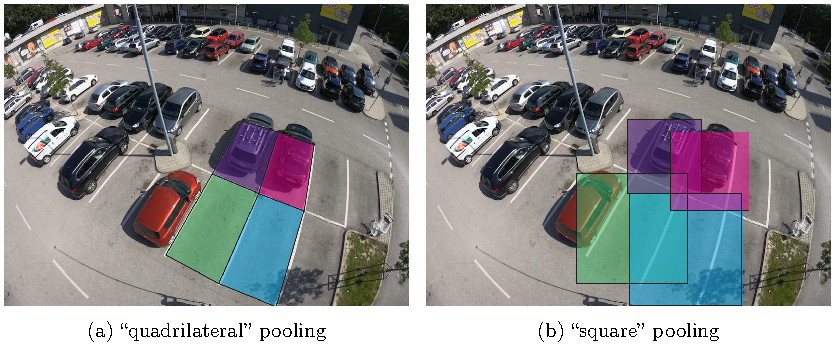
\includegraphics[width=0.75\textwidth]{figures/pooling.pdf}
\caption{Quadrilateral vs.\ square pooling of parking spaces (reproduced
from Marek~\cite{marek2021imagebased}). The quadrilateral region (a) contains only
the target spot's pixels; the bounding square (b) --- geometrically
equivalent to an axis-aligned ROI --- bleeds into
neighboring spots and remains perspective-distorted.}
\label{fig:pooling}
\end{figure}

The pipeline adopts method~(a). Each quadrilateral is passed through
\texttt{order\_corners()}, which enforces a clockwise top-left
$\rightarrow$ top-right $\rightarrow$ bottom-right $\rightarrow$
bottom-left ordering --- without it, \texttt{getPerspectiveTransform}
produces mirrored or twisted warps. The ordered corners define a
homography, and \texttt{warpPerspective} maps the spot to a flat,
top-down $128\times128$ patch. For new cameras without ACPDS-style
annotations, the owner-setup flow (Section~\ref{sec:product}) generates the
quadrilateral layout from uploaded photos; axis-aligned ROIs remain in the
codebase only as a legacy fallback.

\subsection{Stage 2 classifier and training}
\label{sec:classifier}

Three YOLOv8-cls variants were considered, all taking the same
$128\times128$ quadrilateral-warped patch as input and emitting a binary
occupancy score. The nano variant is the deployment target: at 2.7\,M
parameters it has roughly $9\times$ fewer weights than the dataset paper's
ResNet50 (25.6\,M) while taking the identical pooled input, which makes the
accuracy comparison fair.

\begin{table}[H]
\centering\small
\begin{tabular}{lrrl}
\toprule
\textbf{Variant} & \textbf{Params} & \textbf{Size} & \textbf{Role} \\
\midrule
YOLOv8n-cls & 2.7\,M & 2.83\,MB & Primary --- edge deployment \\
YOLOv8s-cls & 6.4\,M & 9.78\,MB & Comparison \\
YOLOv8m-cls & 17\,M & 30.22\,MB & Comparison \\
\bottomrule
\end{tabular}
\caption{Stage 2 classifier variants. All use a $128\times128$
quadrilateral-pooled input and a binary occupied/free head.}
\label{tab:variants}
\end{table}

All variants were trained from scratch on quadrilateral-warped ACPDS
patches with the configuration in Table~\ref{tab:trainconfig}; the
near-balanced class distribution removed the need for class weighting.

\begin{table}[H]
\centering\small
\begin{tabular}{ll}
\toprule
\textbf{Setting} & \textbf{Value} \\
\midrule
Epochs & 50 (patience 20, early stop) \\
Batch size & 64 \\
Optimizer & AdamW, cosine LR schedule \\
LR (initial / final) & 0.001 / 0.00001 \\
Dropout & 0.1 \\
Device & Apple Silicon MPS \\
Augmentation & RandAugment + h-flip + HSV \\
 & jitter + random erasing ($p{=}0.2$) \\
\bottomrule
\end{tabular}
\caption{Stage 2 training configuration.}
\label{tab:trainconfig}
\end{table}

\subsection{Edge inference pipeline}
\label{sec:edge}

The trained \texttt{best.pt} weights are loaded by
\texttt{edge/detect.py}, which runs on still images, image folders, or a
live camera. At startup the script loads the published polygon layout
(from \texttt{GET /map} when a backend is available), warps every spot,
batches the patches through the classifier, and applies temporal
smoothing so a single misclassified frame cannot flip a spot's reported
state. The \texttt{--post} flag pushes the JSON payload to the backend
after each pass:

\noindent
\begin{minipage}{\linewidth}
\begin{lstlisting}
{
  "spots":      { "spot_1": "free", "spot_2": "occupied" },
  "confidence": { "spot_1": 0.91,   "spot_2": 0.84 },
  "timestamp":  "2026-04-21T00:00:00Z"
}
\end{lstlisting}
\end{minipage}

Figure~\ref{fig:detection} shows an annotated output frame, with each
quadrilateral colored by predicted state and labeled with its confidence.
Because only this JSON crosses the network, the reporting path keeps a
measured 99.9\,\% bandwidth reduction relative to a 1080p H.264 stream,
with no camera footage leaving the device.

\begin{figure}[tbp]
\centering
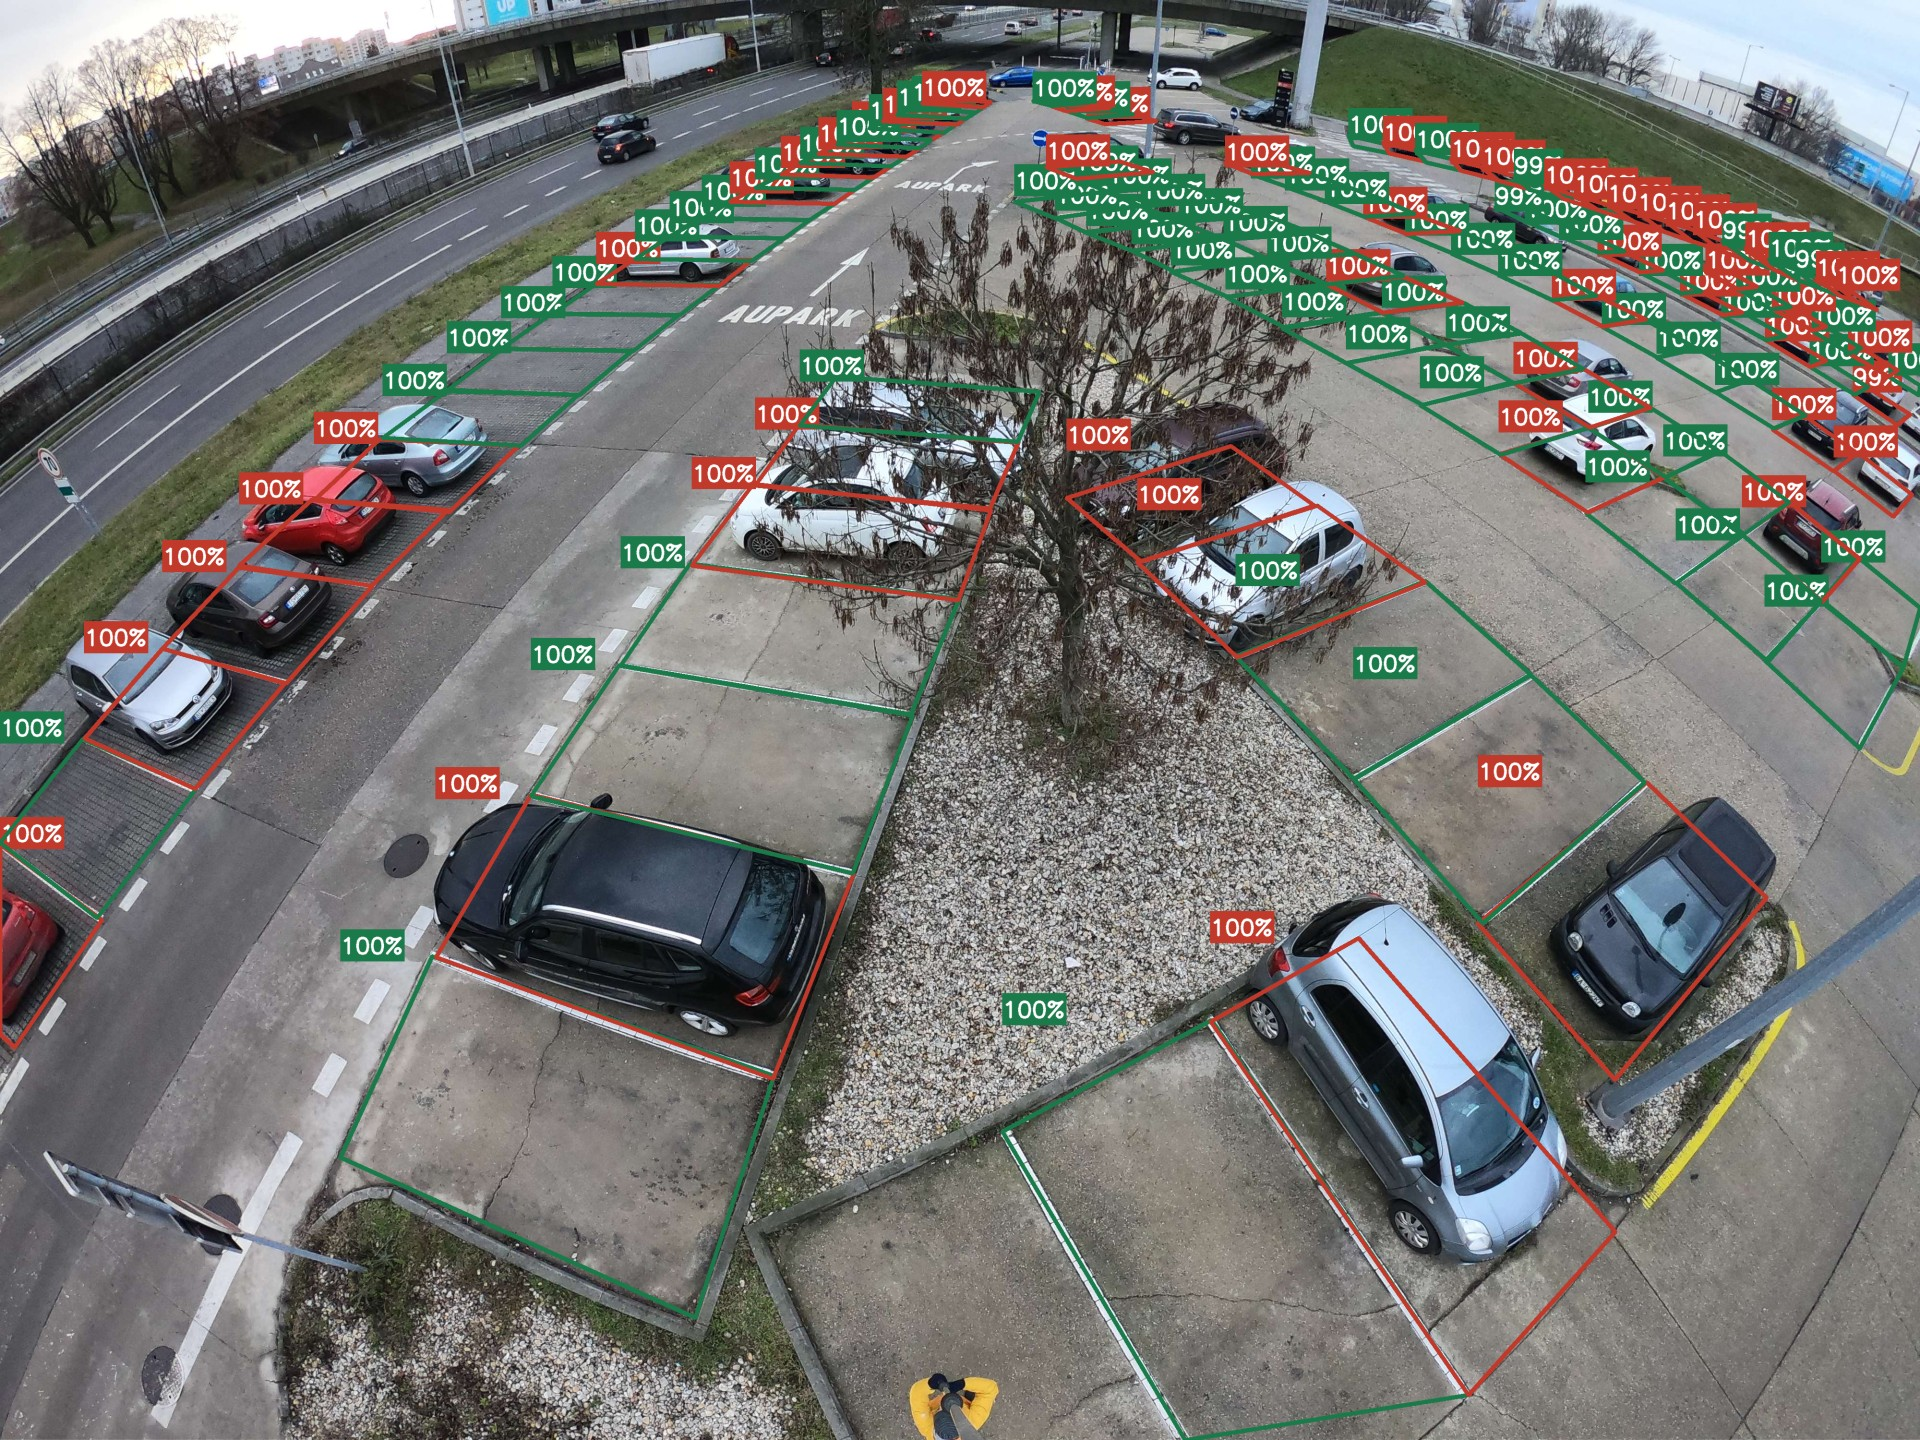
\includegraphics[width=0.78\textwidth]{figures/detection.jpg}
\caption{Annotated edge inference output
(\texttt{runs/output/detection.jpg}). Quadrilateral spot polygons are
colored by predicted state (green free, red occupied) with per-spot
confidence; on this ACPDS lot the promoted classifier reads 70 free /
50 occupied.}
\label{fig:detection}
\end{figure}

\subsection{Backend and software design}
\label{sec:backend}

A FastAPI backend with a SQLite store ties the pieces together. The
edge device posts occupancy to \texttt{POST /update} and clients read it
from \texttt{GET /status}; the lot layout is published with
\texttt{POST /map} (alias \texttt{/layout}) and served from
\texttt{GET /map}, with \texttt{GET /map/background} returning the
bird's-eye-view backdrop. The \emph{Find My Car} flow adds
\texttt{POST /park} (upload a driver photo, run localization, store a
session) and \texttt{GET /find/\{session\_id\}} (return the matched spot
and its corner coordinates). The same published layout drives the edge
runtime, the web map, and the mobile map, so all three stay consistent by
construction.

%%%%%%%%%%%%%%%%%%%%%%%%%%%%%%%%%%%%%%%%%%%%%%%%%%%%%%%%%%%%%%%%%%%%%%%%%%%%%%%%%
\section{Result analyses}
\label{sec:results-analyses}
%%%%%%%%%%%%%%%%%%%%%%%%%%%%%%%%%%%%%%%%%%%%%%%%%%%%%%%%%%%%%%%%%%%%%%%%%%%%%%%%%

\subsection{Dataset: ACPDS}
\label{sec:dataset}

All training and evaluation use ACPDS, the Action-Camera Parking
Dataset~\cite{marek2021imagebased}, captured with a GoPro Hero~6 on a
$\sim$12\,m mast --- a vantage point close to a real lamppost-mounted
camera. It contains 293 high-resolution lot images with 11{,}236 parking
spaces, each annotated as a four-corner quadrilateral rather than a
bounding box, which is exactly what makes the perspective-warp pooling of
Section~\ref{sec:pivot} possible. Crucially, the train / validation / test
splits use \emph{disjoint parking lots} (231 / 35 / 27 images;
7{,}842 / 1{,}904 / 1{,}490 spaces), so test accuracy measures
generalization to lots never seen in training rather than memorization of a
fixed scene --- unlike PKLot~\cite{almeida2015pklot} and CNRPark-EXT, whose
same-lot splits inflate reported accuracy. After warping each quadrilateral
to a $128\times128$ patch, the Stage 2 dataset is near-balanced
($\sim$52\,\% free / 48\,\% occupied: 3{,}902 / 3{,}940 train,
1{,}073 / 831 val, 885 / 605 test, free / occupied). ACPDS is MIT-licensed.

\subsection{Validation accuracy and the retraining gain}
\label{sec:results}

Table~\ref{tab:results} compares the earlier fixed-ROI baseline with the
retrained quadrilateral-warp classifiers on the validation lots, including
a controlled square-crop ablation of the nano variant.

\begin{table}[H]
\centering
\begin{tabular}{llrr}
\toprule
\textbf{Model} & \textbf{Patch extraction} & \textbf{Epochs} &
\textbf{Best top-1 val.\ acc.} \\
\midrule
\multicolumn{4}{l}{\emph{Earlier baseline (rectangular crops, threshold-calibrated)}} \\
YOLOv8m-cls & fixed ROI crops & --- & 90.85\,\%\textsuperscript{a} \\
\midrule
\multicolumn{4}{l}{\emph{Current (quadrilateral-warp retraining)}} \\
YOLOv8n-cls & quadrilateral warp & 50 & \textbf{98.27\,\%} \\
YOLOv8s-cls & quadrilateral warp & 31 & 98.16\,\% \\
YOLOv8m-cls & quadrilateral warp & 50 & 97.95\,\% \\
YOLOv8n-cls & square crop (ablation) & 11 & 96.59\,\% \\
\midrule
ResNet50 (ACPDS paper~\cite{marek2021imagebased}) & quadrilateral warp & --- & $\sim$98\,\% \\
\bottomrule
\end{tabular}
\caption{Stage 2 classification on ACPDS validation lots.
\textsuperscript{a}\,The baseline figure is accuracy at the deployed
threshold 0.3; it is included for trajectory, not as a strictly
like-for-like comparison.}
\label{tab:results}
\end{table}

Three findings stand out. First, the accuracy jump from the earlier
deployment (90.9\,\%) to the current pipeline (98.3\,\%) comes
overwhelmingly from the input representation, not from model capacity:
after the warp normalizes perspective and removes neighboring-spot
pixels, the \emph{smallest} variant wins, and the larger m-variant trails
it. Second, the square-crop ablation isolates the pooling effect directly:
98.27\,\% vs.\ 96.59\,\% is a 1.7-point gap on identical data and
architecture (the square run also converged more slowly and stopped early,
so this is a lower bound at this budget). Third, training is stable ---
Figure~\ref{fig:curves} shows smooth loss decay with the accuracy plateau
reached within roughly 20 epochs, and Figure~\ref{fig:smcurves} shows the
same for the larger variants --- and the confusion matrix in
Figure~\ref{fig:qualitative} shows balanced class performance.

\begin{figure}[tbp]
\centering
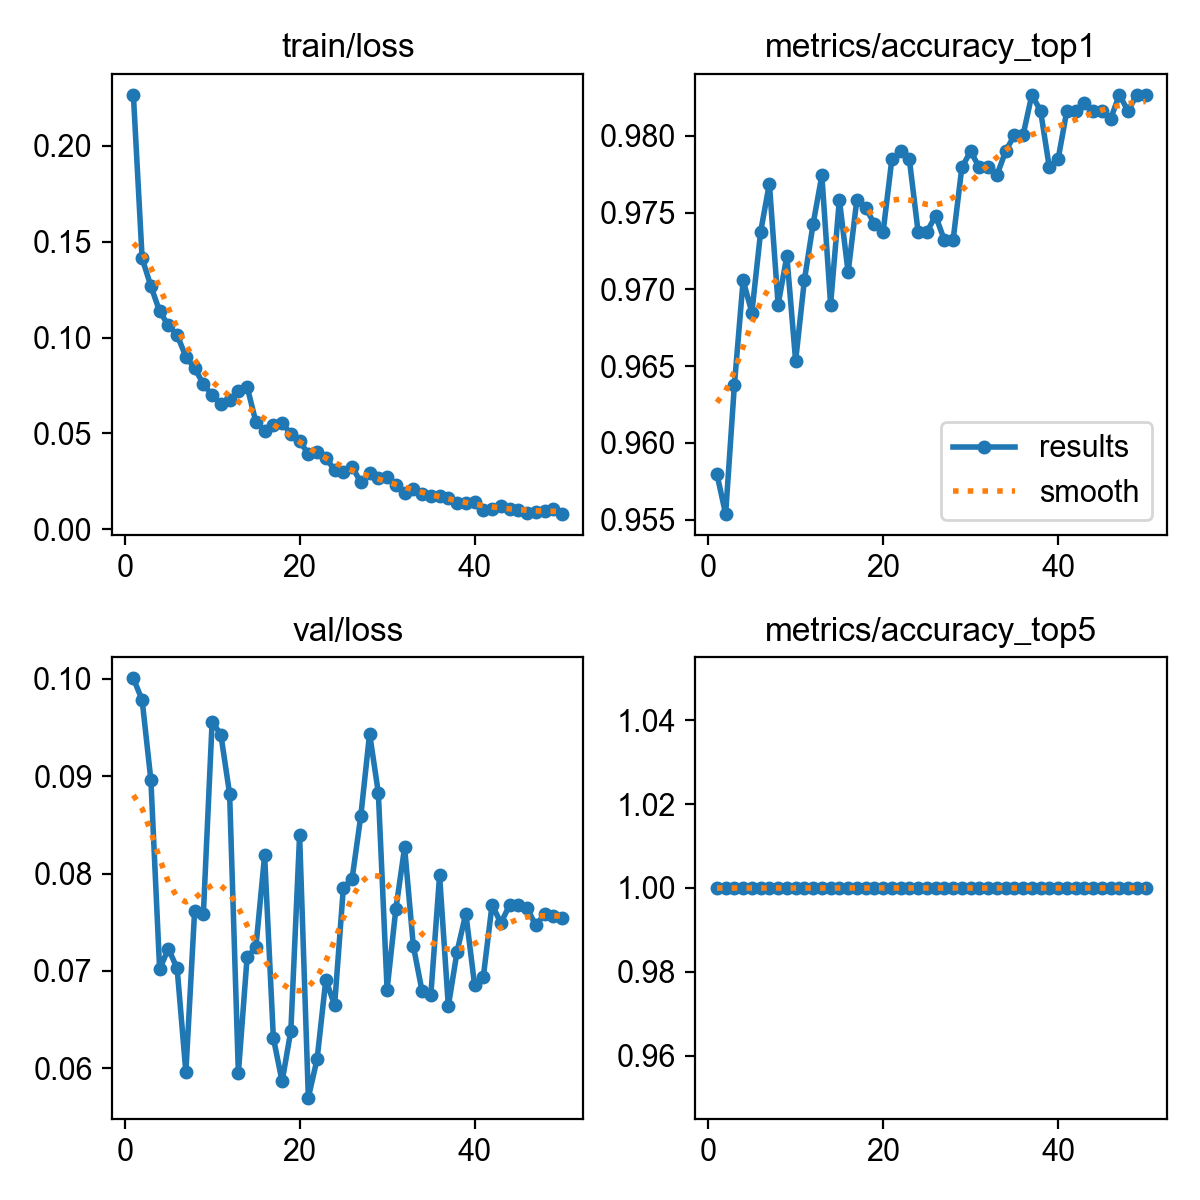
\includegraphics[width=0.78\textwidth]{figures/yolov8n_results.png}
\caption{YOLOv8n-cls training curves on warped ACPDS patches
(\texttt{runs/acpds\_cls/yolov8n\_stage2}): train/validation loss and
top-1 accuracy over 50 epochs.}
\label{fig:curves}
\end{figure}

\begin{figure}[tbp]
\centering
\begin{subfigure}[t]{0.55\textwidth}
  \centering
  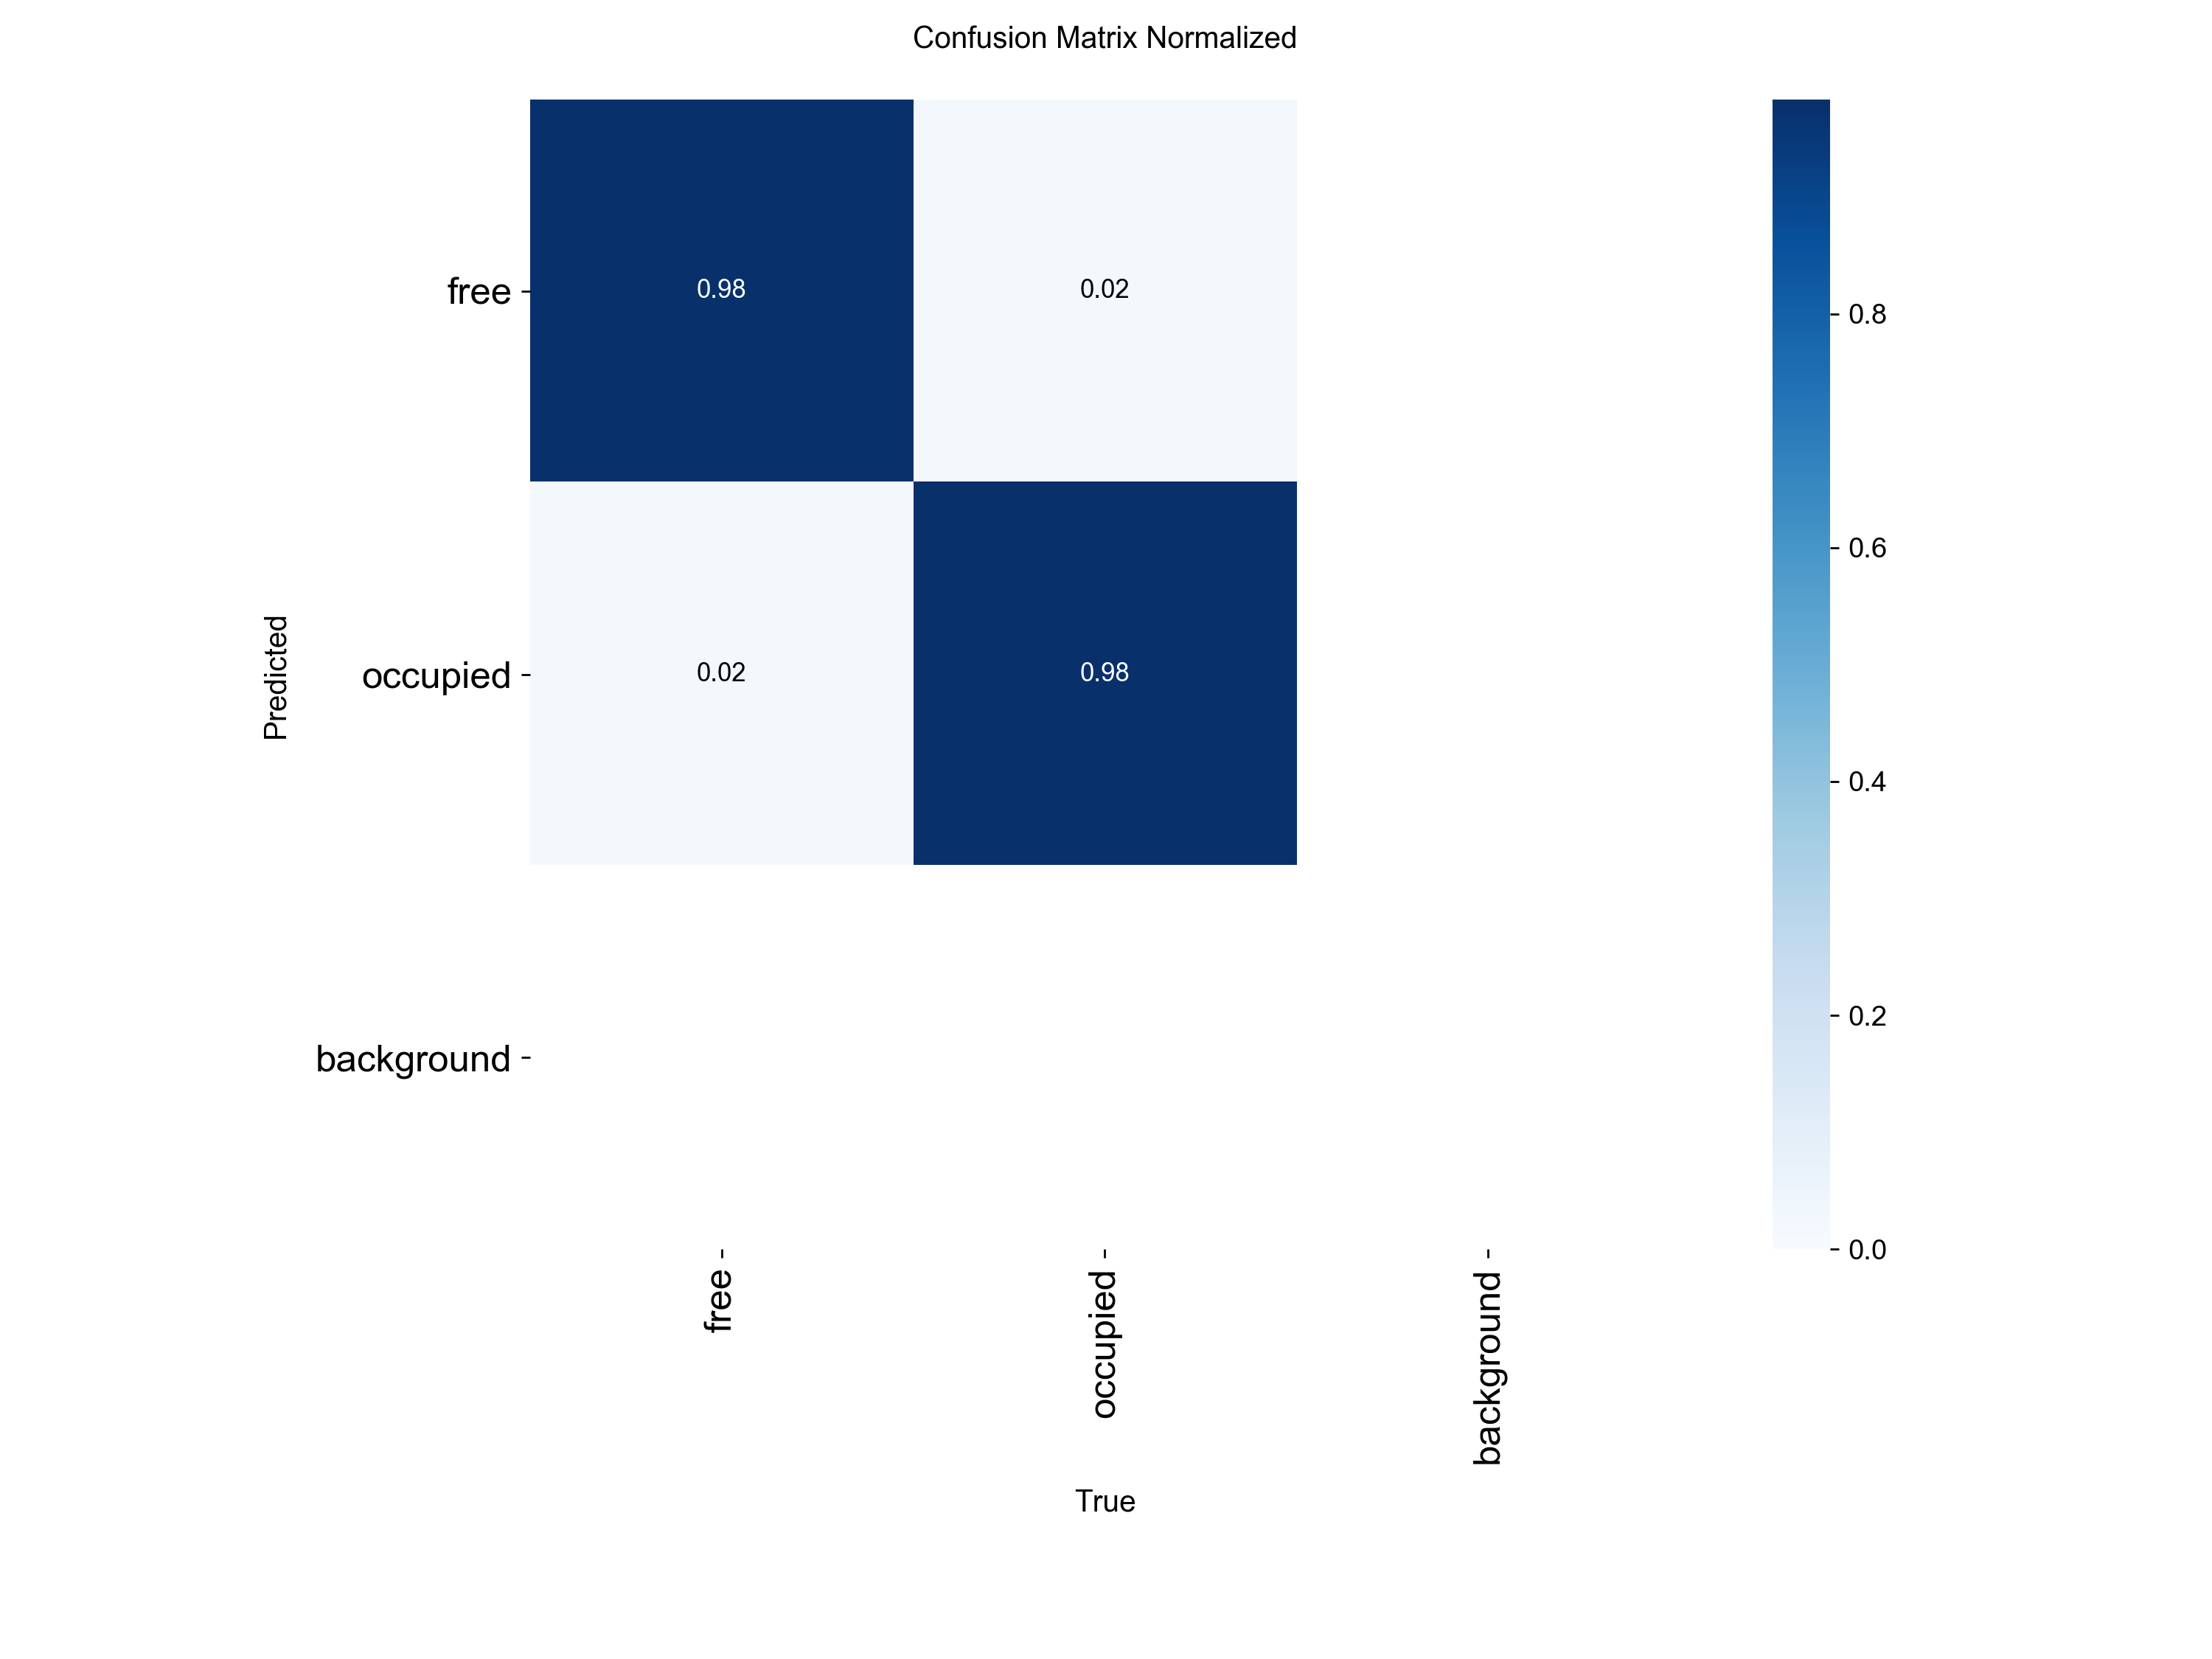
\includegraphics[width=\textwidth]{figures/yolov8n_confusion.png}
  \caption{Normalized confusion matrix.}
\end{subfigure}\hfill
\begin{subfigure}[t]{0.40\textwidth}
  \centering
  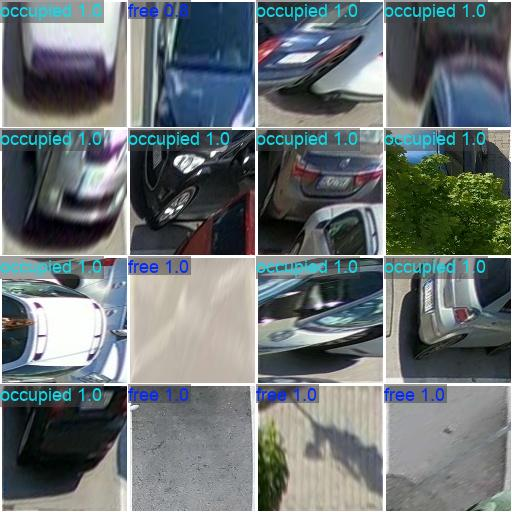
\includegraphics[width=\textwidth]{figures/yolov8n_val_pred.jpg}
  \caption{Validation-batch predictions.}
\end{subfigure}
\caption{YOLOv8n-cls qualitative results. The confusion matrix (a) shows
balanced performance across the \emph{occupied} and \emph{free} classes;
(b) shows predicted labels on warped validation patches.}
\label{fig:qualitative}
\end{figure}

\begin{figure}[tbp]
\centering
\begin{subfigure}[t]{0.49\linewidth}
  \centering
  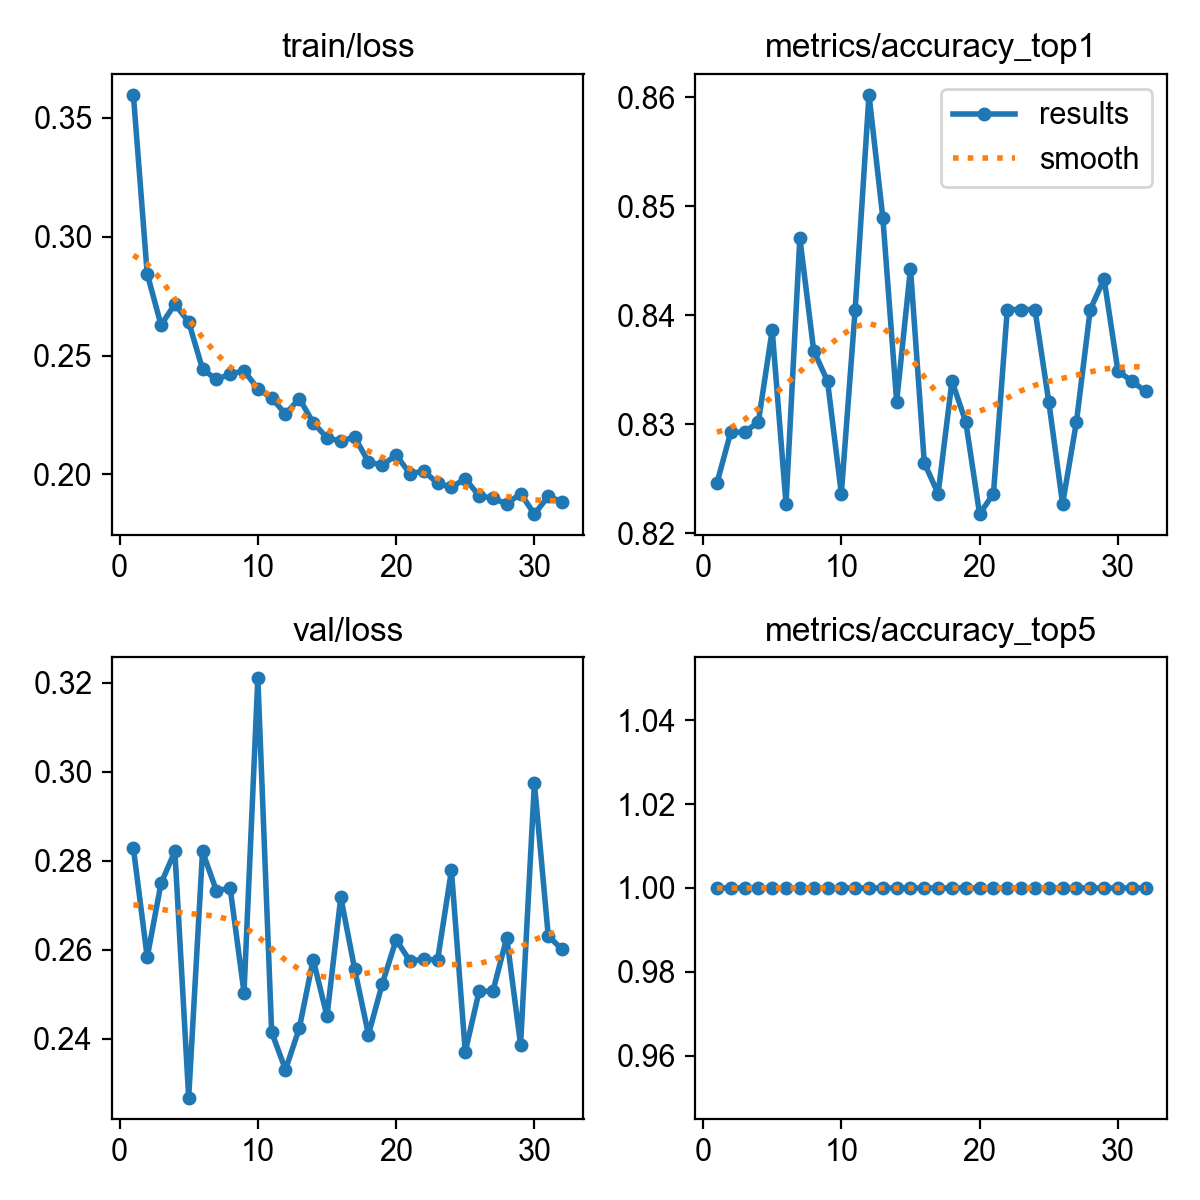
\includegraphics[width=\textwidth]{figures/w11_yolov8s_curves.png}
  \caption{YOLOv8s-cls (32 epochs).}
\end{subfigure}\hfill
\begin{subfigure}[t]{0.49\linewidth}
  \centering
  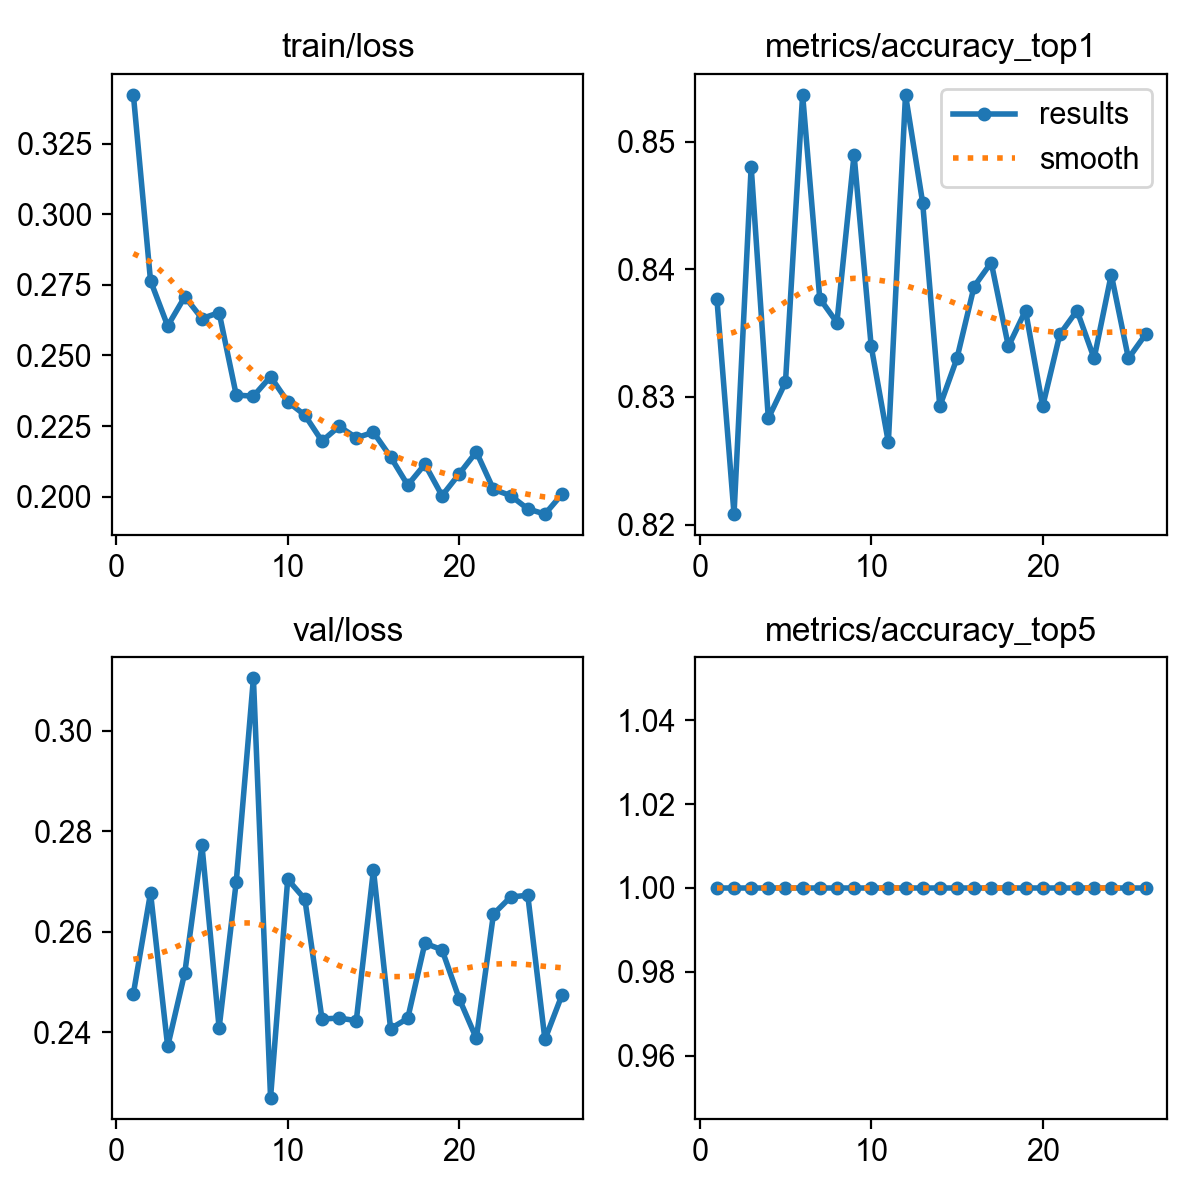
\includegraphics[width=\textwidth]{figures/w11_yolov8m_curves.png}
  \caption{YOLOv8m-cls (26 epochs).}
\end{subfigure}
\caption{Training curves for the comparison variants: train/validation
loss and validation top-1 accuracy.}
\label{fig:smcurves}
\end{figure}

\subsection{Test-split model comparison}

Table~\ref{tab:testcompare} reports every trained model on the held-out
ACPDS test split --- 1{,}490 patches from parking lots in neither the
training nor the validation sets, the number that measures genuine
generalization --- alongside the paper's ResNet50 baselines and the INT8
ONNX export. The key finding is that \textbf{YOLOv8n-cls outperforms the
larger s and m variants on the test split} despite having 2.4--6.3$\times$
fewer parameters, and the INT8 export reproduces the PyTorch accuracy
exactly --- quantization introduces no measurable loss at this model size.
The 98\,\% paper target on the test split is narrowly missed by 0.28\,pp;
the evidence in the following subsections points to patch quality and
distribution shift, not model capacity, as the remaining bottleneck.

\begin{table}[H]
\centering\footnotesize
\setlength{\tabcolsep}{4pt}
\begin{tabular}{llrrrr}
\toprule
\textbf{Model} & \textbf{Pool} & \textbf{Test} & \textbf{Val} &
\textbf{Test F1} & \textbf{Params} \\
\midrule
ResNet50 R-CNN\textsuperscript{$\ast$} & sq. & 97.97 & 98.38 & --- & 25.6\,M \\
ResNet50 FPN\textsuperscript{$\ast$} & sq. & 98.51 & 98.58 & --- & 25.6\,M \\
\midrule
YOLOv8n-cls (prom.) & quad & \textbf{97.72} & 98.27 & 0.9715 & 2.7\,M \\
YOLOv8s-cls & quad & 96.91 & 98.16 & 0.9615 & 6.4\,M \\
YOLOv8m-cls & quad & 97.38 & 97.95 & 0.9672 & 17\,M \\
YOLOv8n INT8 ONNX & quad & 97.72 & 98.27 & 0.9715 & 2.7\,M \\
YOLOv8n-cls (abl.) & sq. & 96.38 & --- & 0.9559 & 2.7\,M \\
\bottomrule
\end{tabular}
\caption{Test-split results on ACPDS (1{,}490 unseen-lot patches).
Accuracies in \%. \textsuperscript{$\ast$}\,ResNet50 figures from
Table~1 of Marek~\cite{marek2021imagebased}.}
\label{tab:testcompare}
\end{table}

\subsection{Validation vs.\ test gap}

All three variants show a small, consistent drop from validation to test
(Table~\ref{tab:valtestgap}, Figure~\ref{fig:valtestgap}): on average
0.79\,pp in accuracy and 3.27\,pp in recall. The consistency across model
sizes rules out model-specific overfitting and points to distribution
shift between the validation and test lots. The recall drop exceeding the
accuracy drop matches the deployed error mode --- occupied spots are
occasionally missed on border-heavy or partial-vehicle patches in the
harder test lots --- and the larger s/m classifiers do not close the gap.

\begin{table}[H]
\centering\small
\setlength{\tabcolsep}{4pt}
\begin{tabular}{lrrrrr}
\toprule
\textbf{Model} & \textbf{Val} & \textbf{Test} & \textbf{$\Delta$} &
\textbf{Val R} & \textbf{Test R} \\
\midrule
YOLOv8n-cls & 98.27 & 97.72 & $-0.55$ & 98.19 & 95.70 \\
YOLOv8s-cls & 98.16 & 96.91 & $-1.25$ & 98.56 & 94.88 \\
YOLOv8m-cls & 97.95 & 97.38 & $-0.57$ & 98.68 & 95.04 \\
\bottomrule
\end{tabular}
\caption{Validation vs.\ test accuracy and recall (\%). $\Delta$ is the
accuracy delta; R denotes recall.}
\label{tab:valtestgap}
\end{table}

\begin{figure}[tbp]
\centering
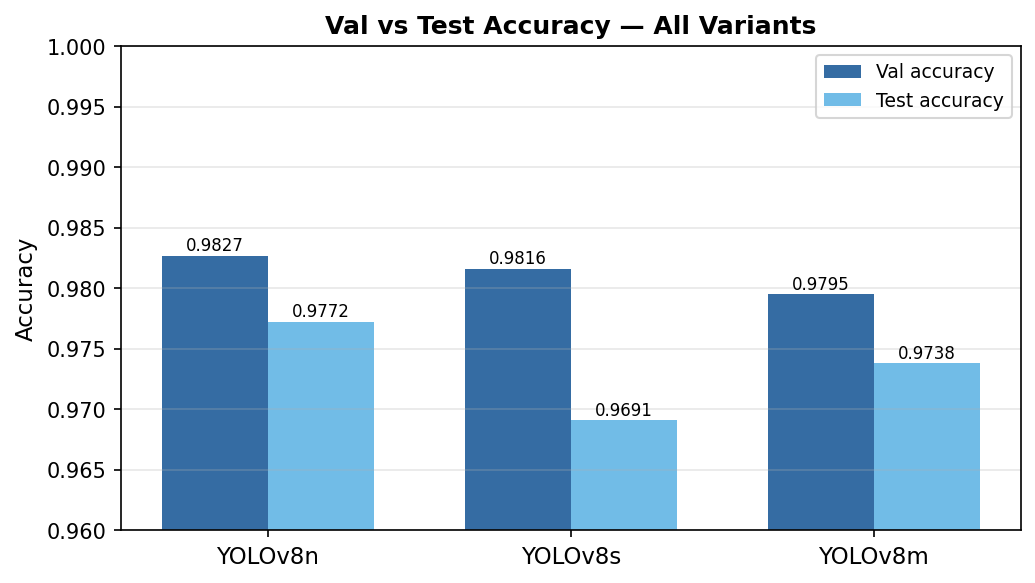
\includegraphics[width=0.75\linewidth]{figures/w11_val_test_gap.png}
\caption{Validation vs.\ test accuracy across the three YOLOv8 variants.
Drops are modest and consistent, indicating distribution shift rather
than overfitting.}
\label{fig:valtestgap}
\end{figure}

\subsection{Confusion matrix and PR curve}

Figure~\ref{fig:cmtest} shows the promoted YOLOv8n-cls confusion matrix on
the test split. The dominant error mode is false negatives: 26 occupied
spaces predicted free (4.3\,\% of occupied), versus only 8 false
positives (0.9\,\% of free). This is the expected pattern for ACPDS at
lamppost height --- partially visible vehicles and small bumper/wheel
fragments inside the warped quadrilateral --- and it shows the model is
conservative about declaring a space occupied. Table~\ref{tab:cmmetrics}
gives the per-class metrics.

\begin{figure}[tbp]
\centering
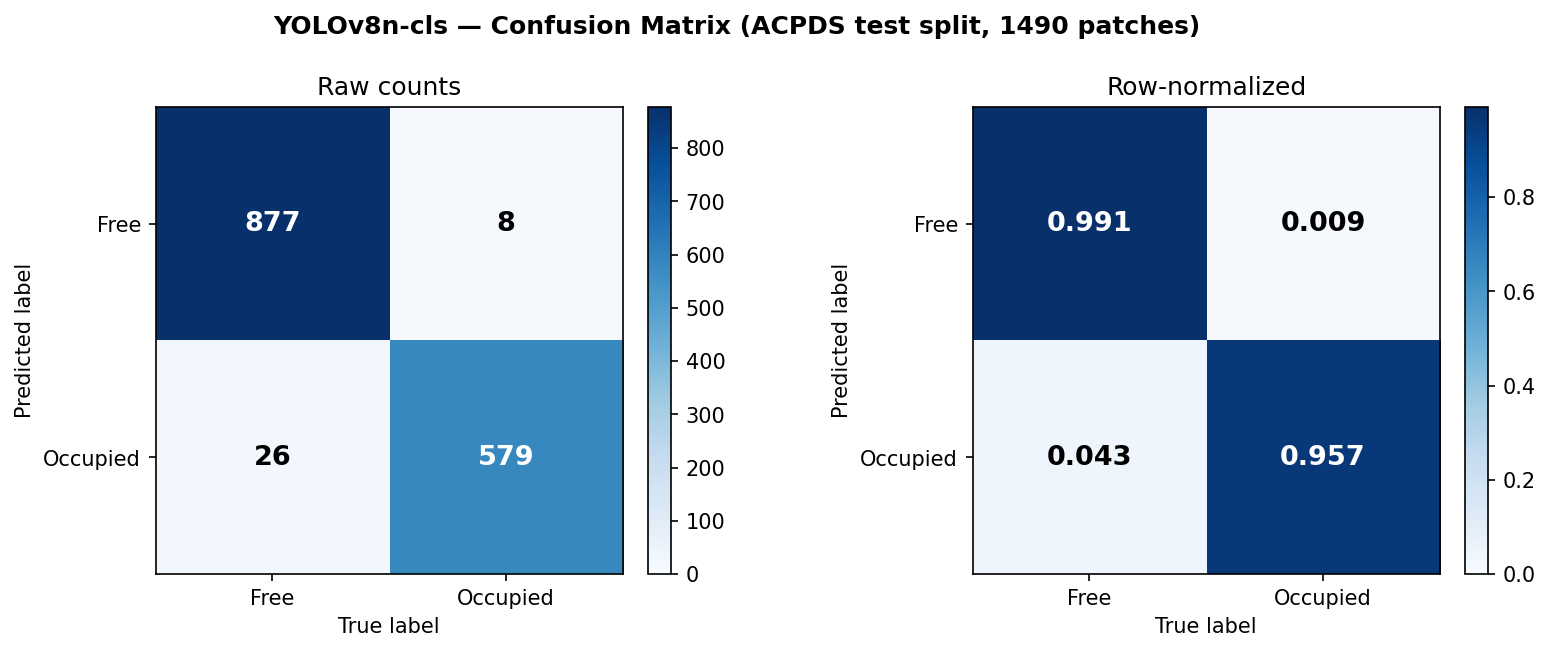
\includegraphics[width=0.95\linewidth]{figures/gen_confusion_test.png}
\caption{YOLOv8n-cls confusion matrix on the test split. Left: raw
counts ($\text{TN}=877$, $\text{FP}=8$, $\text{FN}=26$,
$\text{TP}=579$). Right: row-normalized. Regenerated directly from the
promoted checkpoint by \texttt{ml/make\_report\_figures.py}
(\texttt{make figures}).}
\label{fig:cmtest}
\end{figure}

\begin{table}[H]
\centering\small
\begin{tabular}{lrrr}
\toprule
\textbf{Metric} & \textbf{Free} & \textbf{Occupied} & \textbf{Overall} \\
\midrule
Precision & 0.9712 & 0.9864 & --- \\
Recall    & 0.9910 & 0.9570 & --- \\
F1        & 0.9810 & 0.9715 & 0.9762 (macro) \\
Support   & 885    & 605    & 1490 \\
\bottomrule
\end{tabular}
\caption{Per-class test metrics for the promoted YOLOv8n-cls model.}
\label{tab:cmmetrics}
\end{table}

The precision--recall curve (Figure~\ref{fig:prcurve}) confirms a
high-precision operating region. At the default threshold of 0.5 recall
is 0.957; raising the threshold toward 0.7--0.8 would trade recall for a
marginal precision gain. For a live system where false \emph{occupied}
signals frustrate drivers more than missed free spaces, operating near
threshold 0.5 is the right trade-off.

\begin{figure}[tbp]
\centering
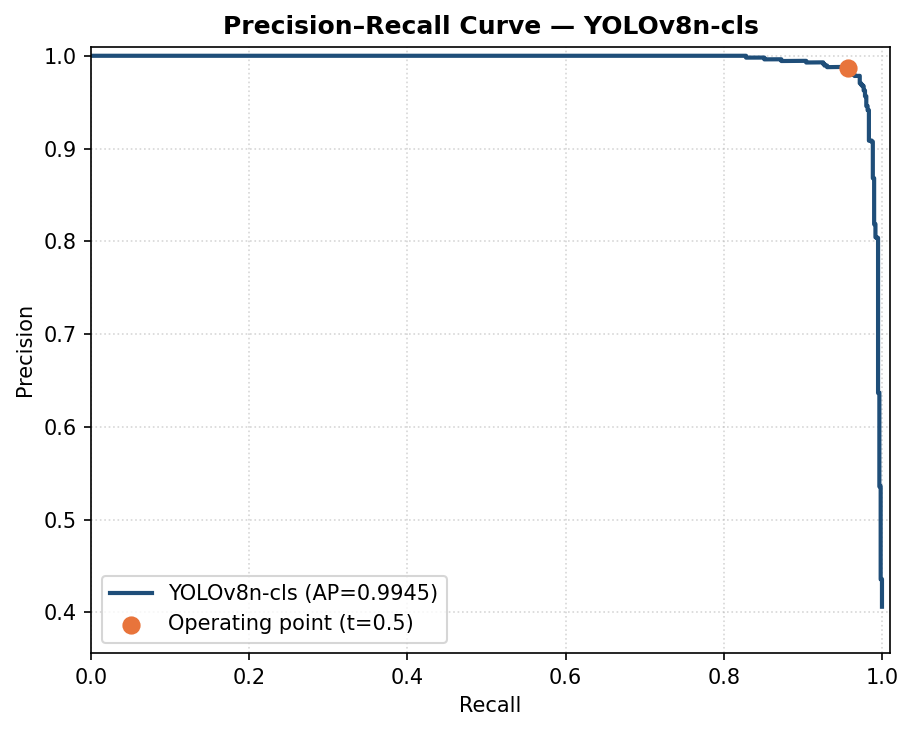
\includegraphics[width=0.62\linewidth]{figures/gen_pr_curve.png}
\caption{Precision--recall curve for YOLOv8n-cls on the test split
(average precision 0.9945); the threshold-0.5 operating point is marked.
Regenerated from the promoted checkpoint by
\texttt{ml/make\_report\_figures.py} (\texttt{make figures}).}
\label{fig:prcurve}
\end{figure}

\subsection{Per-weather accuracy}

The test split was bucketed into sunny, overcast, and low-light thirds by
image luminance (HSV V-channel tertiles). Accuracy degrades monotonically
from sunny (98.94\,\%) to low-light (96.63\,\%), a 2.3\,pp drop
(Table~\ref{tab:weather}, Figure~\ref{fig:weather}). The effect is
asymmetric: under low-light, precision actually \emph{rises} to 99.6\,\%
while recall falls to 93.5\,\%, i.e.\ the model becomes very conservative
--- lower contrast and reduced texture make partially visible vehicles
harder to distinguish from empty asphalt in the warped patch. Luminance-
aware augmentation is a natural way to close this gap.

\begin{table}[H]
\centering\small
\setlength{\tabcolsep}{4pt}
\begin{tabular}{lrrrr}
\toprule
\textbf{Condition} & \textbf{N} & \textbf{Acc.} & \textbf{Prec.} &
\textbf{Recall} \\
\midrule
Sunny ($V>124.5$)        & 470 & 98.94 & 98.32 & 98.88 \\
Overcast ($112.9$--$124.5$) & 486 & 97.74 & 97.53 & 95.76 \\
Low-light ($V<112.9$)    & 534 & 96.63 & 99.59 & 93.51 \\
\bottomrule
\end{tabular}
\caption{Per-weather test metrics (\%) for YOLOv8n-cls, bucketed by
image luminance.}
\label{tab:weather}
\end{table}

\begin{figure}[tbp]
\centering
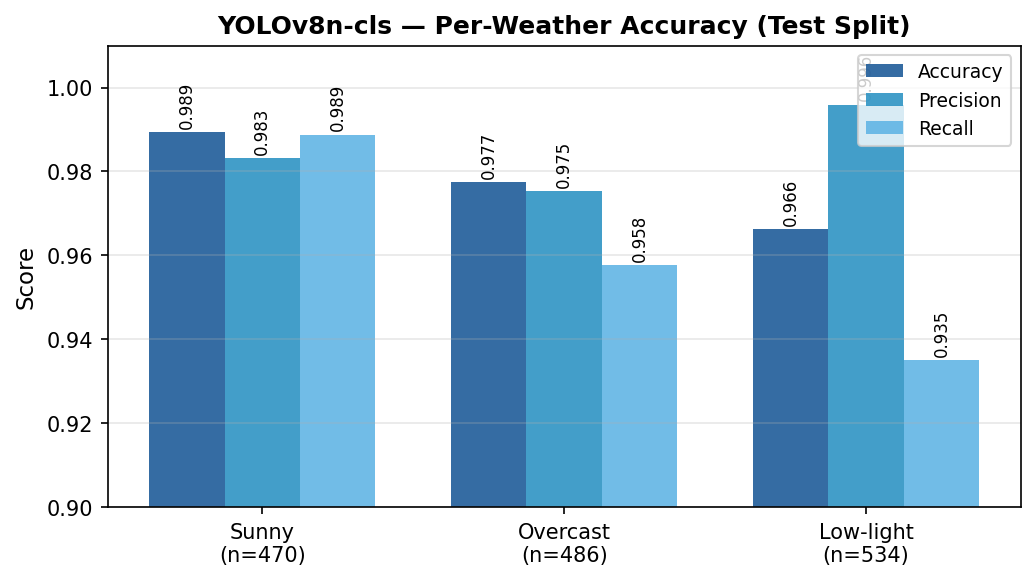
\includegraphics[width=0.75\linewidth]{figures/w11_per_weather.png}
\caption{Per-weather accuracy, precision, and recall for YOLOv8n-cls on
the test split.}
\label{fig:weather}
\end{figure}

\subsection{Pooling comparison on the test split}

The validation ablation in Table~\ref{tab:results} is corroborated on the
held-out test split: the same YOLOv8n-cls architecture trained on
quadrilateral- vs.\ square-pooled patches
(Table~\ref{tab:poolcompare}, Figure~\ref{fig:poolcompare}) gives
quadrilateral pooling a $+1.34$\,pp accuracy, $+4.13$\,pp precision, and
$+1.56$\,pp F1 advantage. Square pooling wins only on recall
($+0.99$\,pp), because the surrounding context in the bounding square
occasionally helps detect partially visible vehicles near the spot edges
--- but that same context injects noise from neighboring spots and
degrades precision, the costlier error here.

\begin{table}[H]
\centering\small
\setlength{\tabcolsep}{4pt}
\begin{tabular}{lrrrr}
\toprule
\textbf{Pooling} & \textbf{Acc.} & \textbf{Prec.} & \textbf{Recall} &
\textbf{F1} \\
\midrule
Quadrilateral (a) & \textbf{97.72} & \textbf{98.64} & 95.70 & \textbf{97.15} \\
Square (b)        & 96.38 & 94.51 & \textbf{96.69} & 95.59 \\
\midrule
$\Delta$ (sq.\ $-$ quad) & $-1.34$ & $-4.13$ & $+0.99$ & $-1.56$ \\
\bottomrule
\end{tabular}
\caption{Quadrilateral vs.\ square pooling on the test split (\%), same
architecture and data.}
\label{tab:poolcompare}
\end{table}

\begin{figure}[tbp]
\centering
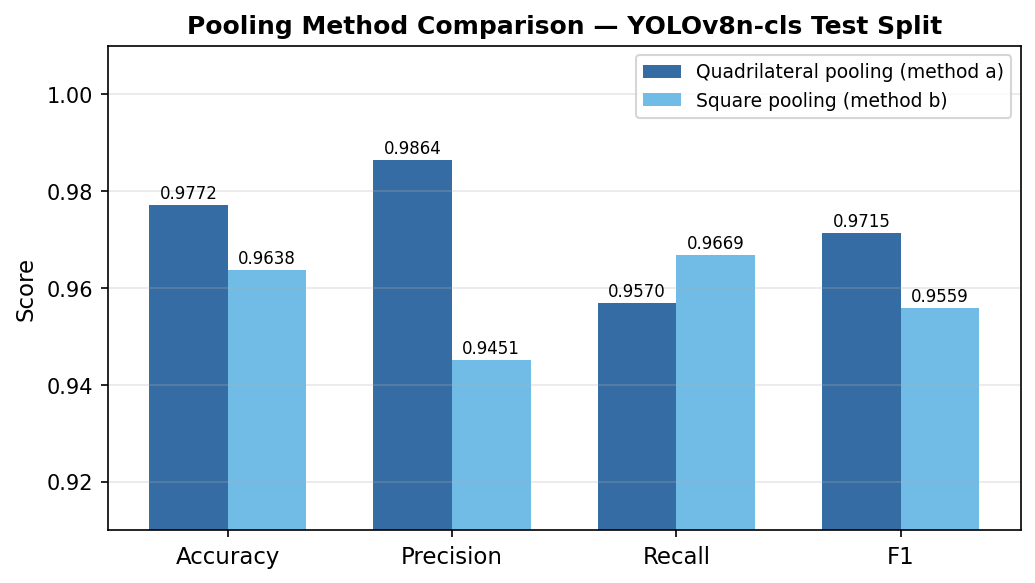
\includegraphics[width=0.85\linewidth]{figures/w11_pooling_compare.png}
\caption{Quadrilateral vs.\ square pooling on the test split. Quad wins
on all metrics except recall.}
\label{fig:poolcompare}
\end{figure}

Notably, this reverses the \emph{direction} of ACPDS Table~2, where
square pooling beat quadrilateral pooling for the paper's R-CNN
architecture. The reversal is consistent with the architectural
difference: R-CNN benefits from surrounding context through its backbone,
whereas YOLOv8-cls sees only the single patch, so a cleaner
perspective-corrected input is more valuable to it.

\subsection{Find My Car localization accuracy}
\label{sec:fmc-eval}

\emph{Find My Car} matches SIFT features from a driver's photo against
per-spot reference images, with FLANN matching and RANSAC homography
verification; the spot with the highest inlier count is the top-1
prediction and the inlier count is the confidence. It runs on CPU only and
needs no training. SIFT-only is the final scope for this submission: it
meets the targets without training, so the MobileNetV3 embedding path
(documented as an optional future upgrade for day/night robustness) is
intentionally out of scope.

Localization was evaluated on a labelled set of 21 night-overhead photos
(\texttt{query\_set.night\_overhead.json}), including the three reference
timestamps as sanity-check queries. The pipeline scored 21/21 on both
top-1 and top-3, comfortably clearing the targets (Table~\ref{tab:fmc}).
The $\sim$536\,ms average is marginally above the 500\,ms target, but the
target is conservative for this feature: \emph{Find My Car} runs
\emph{once} on arrival and once on return, not in a continuous loop, so
536\,ms is a single user-facing wait rather than a throughput constraint.

\begin{table}[H]
\centering\small
\begin{tabular}{lll}
\toprule
\textbf{Metric} & \textbf{Target} & \textbf{Result (21 queries)} \\
\midrule
Top-1 accuracy & $>85\,\%$ & 100\,\% (21/21) \\
Top-3 accuracy & $>95\,\%$ & 100\,\% (21/21) \\
Avg.\ runtime  & $<500$\,ms & $\sim$536\,ms \\
GPU required   & No & CPU only --- met \\
\bottomrule
\end{tabular}
\caption{Find My Car localization results on the labelled night-overhead
query set (21 queries).}
\label{tab:fmc}
\end{table}

\subsection{Inference speed and deployment}
\label{sec:speed-sub}

Stage 2 inference was benchmarked on the edge device (Apple Silicon
MacBook) over 200 timed single-patch inferences after 10 warmup
iterations per backend (Table~\ref{tab:speed}). Every backend runs far
above the system's needs: the edge runtime posts occupancy at roughly
0.5\,Hz, so even the slowest path (PyTorch MPS at 155\,FPS) has a
$\sim$300$\times$ throughput margin. Two results are worth noting. First,
CPU \emph{outpaces} MPS for these $128\times128$ patches (207 vs.\
155\,FPS): the patch is so small that GPU dispatch overhead dominates and
the device never saturates, so the MPS advantage that shows up on
full-frame models disappears here. Second, the Core ML INT8 export --- the
actual quantized Apple-Silicon deployment artifact --- is fastest at
858\,FPS (1.2\,ms), with no accuracy loss relative to the PyTorch
checkpoint.

\begin{table}[H]
\centering\small
\begin{tabular}{lrr}
\toprule
\textbf{Backend} & \textbf{Latency (ms)} & \textbf{FPS} \\
\midrule
PyTorch MPS                     & 6.5 & 155 \\
PyTorch CPU                     & 4.8 & 207 \\
ONNX FP32 (CPU)                 & 3.3 & 302 \\
Core ML INT8 (Apple Silicon)\textsuperscript{$\ast$} & \textbf{1.2} & \textbf{858} \\
\bottomrule
\end{tabular}
\caption{Measured Stage 2 (\texttt{yolov8n-cls}, $128\times128$)
inference speed by backend: mean of 200 single-patch runs after 10
warmups. \textsuperscript{$\ast$}\,The ONNX INT8 export could not be
benchmarked on the installed ONNX Runtime (the CPU execution provider
lacks a \texttt{ConvInteger} implementation), so the Core ML INT8 export
--- the deployed quantized artifact --- is reported in its place.}
\label{tab:speed}
\end{table}

%%%%%%%%%%%%%%%%%%%%%%%%%%%%%%%%%%%%%%%%%%%%%%%%%%%%%%%%%%%%%%%%%%%%%%%%%%%%%%%%%
\section{Application description}
\label{sec:product}
%%%%%%%%%%%%%%%%%%%%%%%%%%%%%%%%%%%%%%%%%%%%%%%%%%%%%%%%%%%%%%%%%%%%%%%%%%%%%%%%%

The product is delivered as a web app (React + Leaflet) and a mobile app
(React Native / Expo) over the FastAPI backend of
Section~\ref{sec:backend}. The platform split is deliberate: owner setup is
web-only, \emph{Find My Car} is mobile-only, and the live occupancy map
ships on both.

\subsection{Owner setup (web)}

The owner uploads reference photos of the lot, the layout is generated as
quadrilateral spot polygons, and the owner publishes it (with a
bird's-eye-view background) via \texttt{POST /map}. This is the one-time
configuration step that every other screen depends on.

\begin{figure}[H]
\centering
\uiplaceholder{ui_owner_setup.png}
% \includegraphics[width=\linewidth]{figures/ui_owner_setup.png}
\caption{Owner setup (web): photo upload and the generated quadrilateral
layout published as the lot map.}
\label{fig:ui-owner}
\end{figure}

\subsection{Live occupancy map (web and mobile)}

Both clients poll \texttt{GET /status} and color each published spot by
its current state, with a free / occupied / total summary. The web map uses
Leaflet polygon overlays; the mobile map renders the same layout as
coordinate-accurate SVG polygons with pinch-to-zoom and pan. Counts are
scoped to the active layout's spot IDs (see Section~\ref{sec:casestudy}).

\begin{figure}[H]
\centering
\begin{subfigure}[t]{0.49\linewidth}
  \centering
  \uiplaceholder{ui_web_map.png}
  % 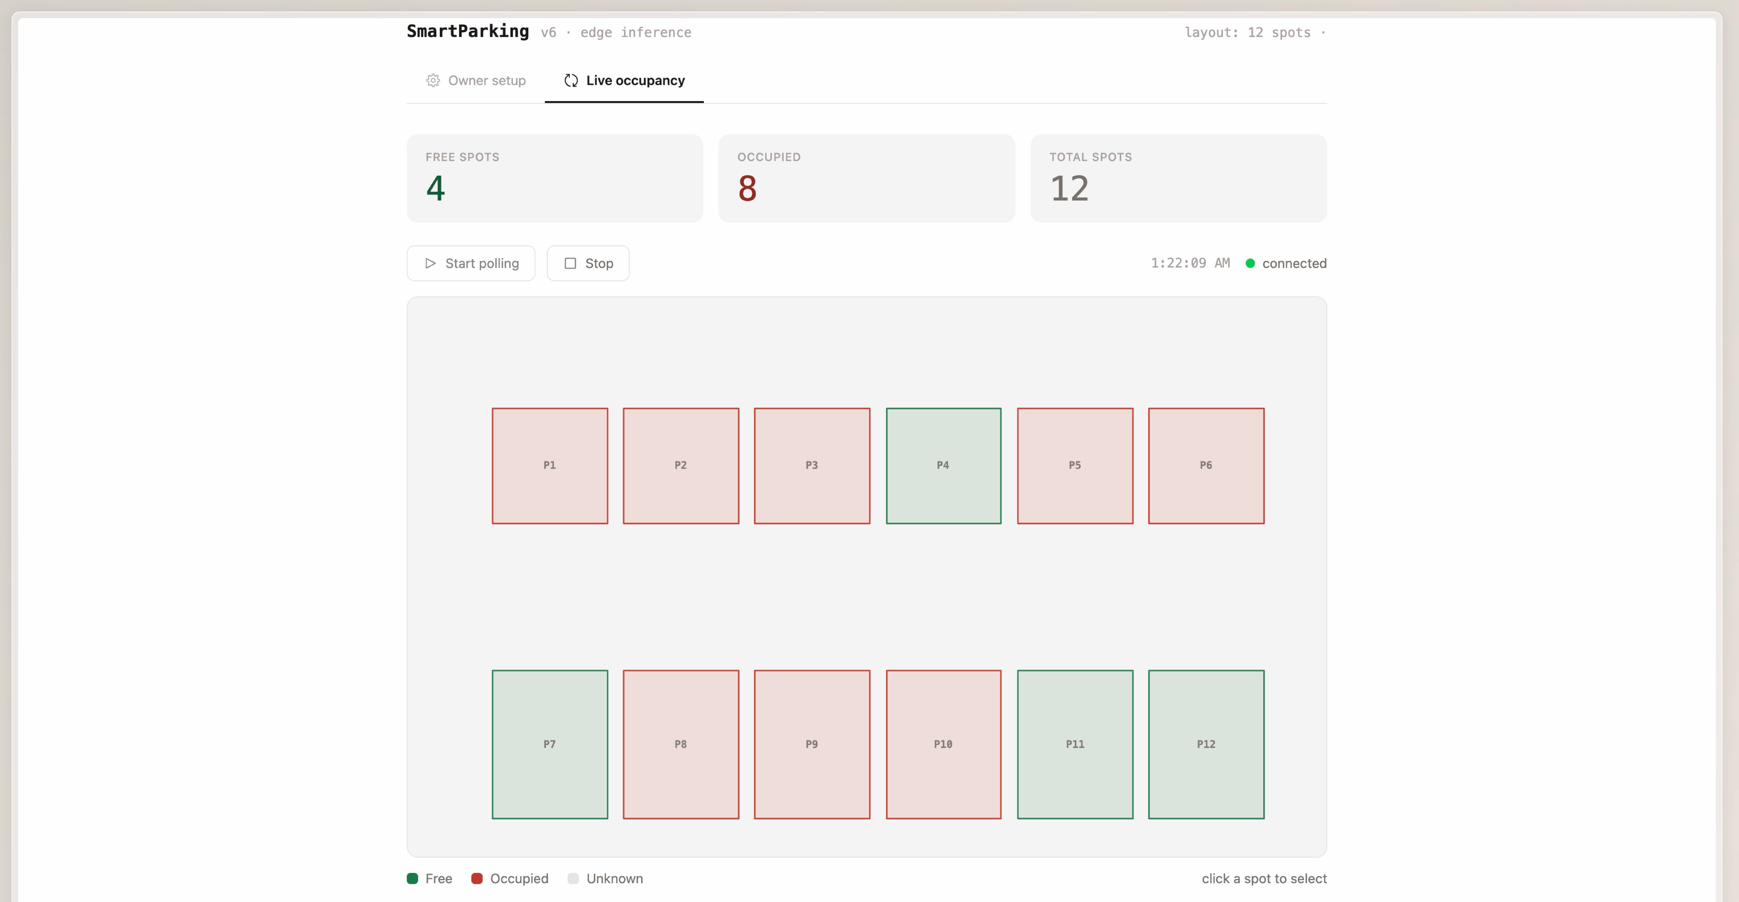
\includegraphics[width=\linewidth]{figures/ui_web_map.png}
  \caption{Web live occupancy map.}
\end{subfigure}\hfill
\begin{subfigure}[t]{0.49\linewidth}
  \centering
  \uiplaceholder{ui_mobile_map.png}
  % 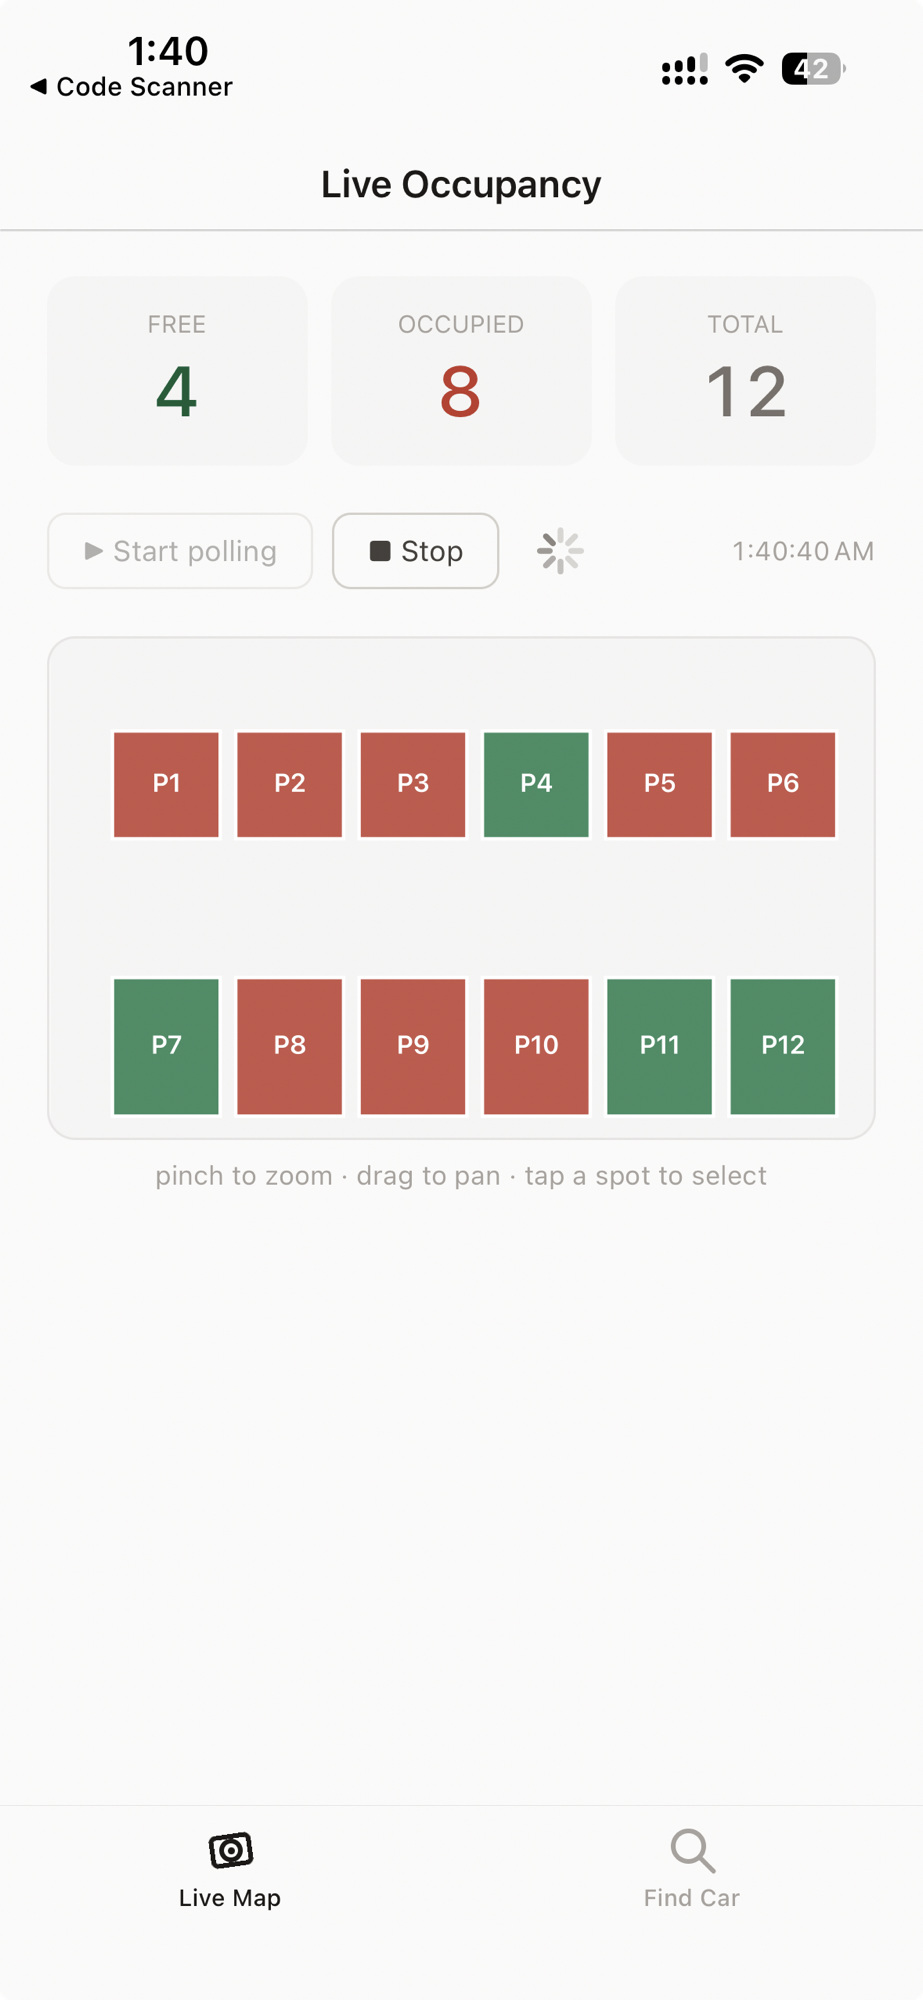
\includegraphics[width=\linewidth]{figures/ui_mobile_map.png}
  \caption{Mobile live occupancy map.}
\end{subfigure}
\caption{Live occupancy map on web (Leaflet) and mobile (SVG + gestures);
spots are colored green for free and red for occupied.}
\label{fig:ui-map}
\end{figure}

\subsection{Find My Car (mobile)}

On arrival the driver taps \emph{Park Here}; the app uploads a photo to
\texttt{POST /park}, which localizes it and returns a \texttt{session\_id}.
Later the driver taps \emph{Find My Car}; the app calls
\texttt{GET /find/\{session\_id\}} and highlights the matched spot in amber
on the map.

\begin{figure}[H]
\centering
\uiplaceholder{ui_find_my_car.png}
% 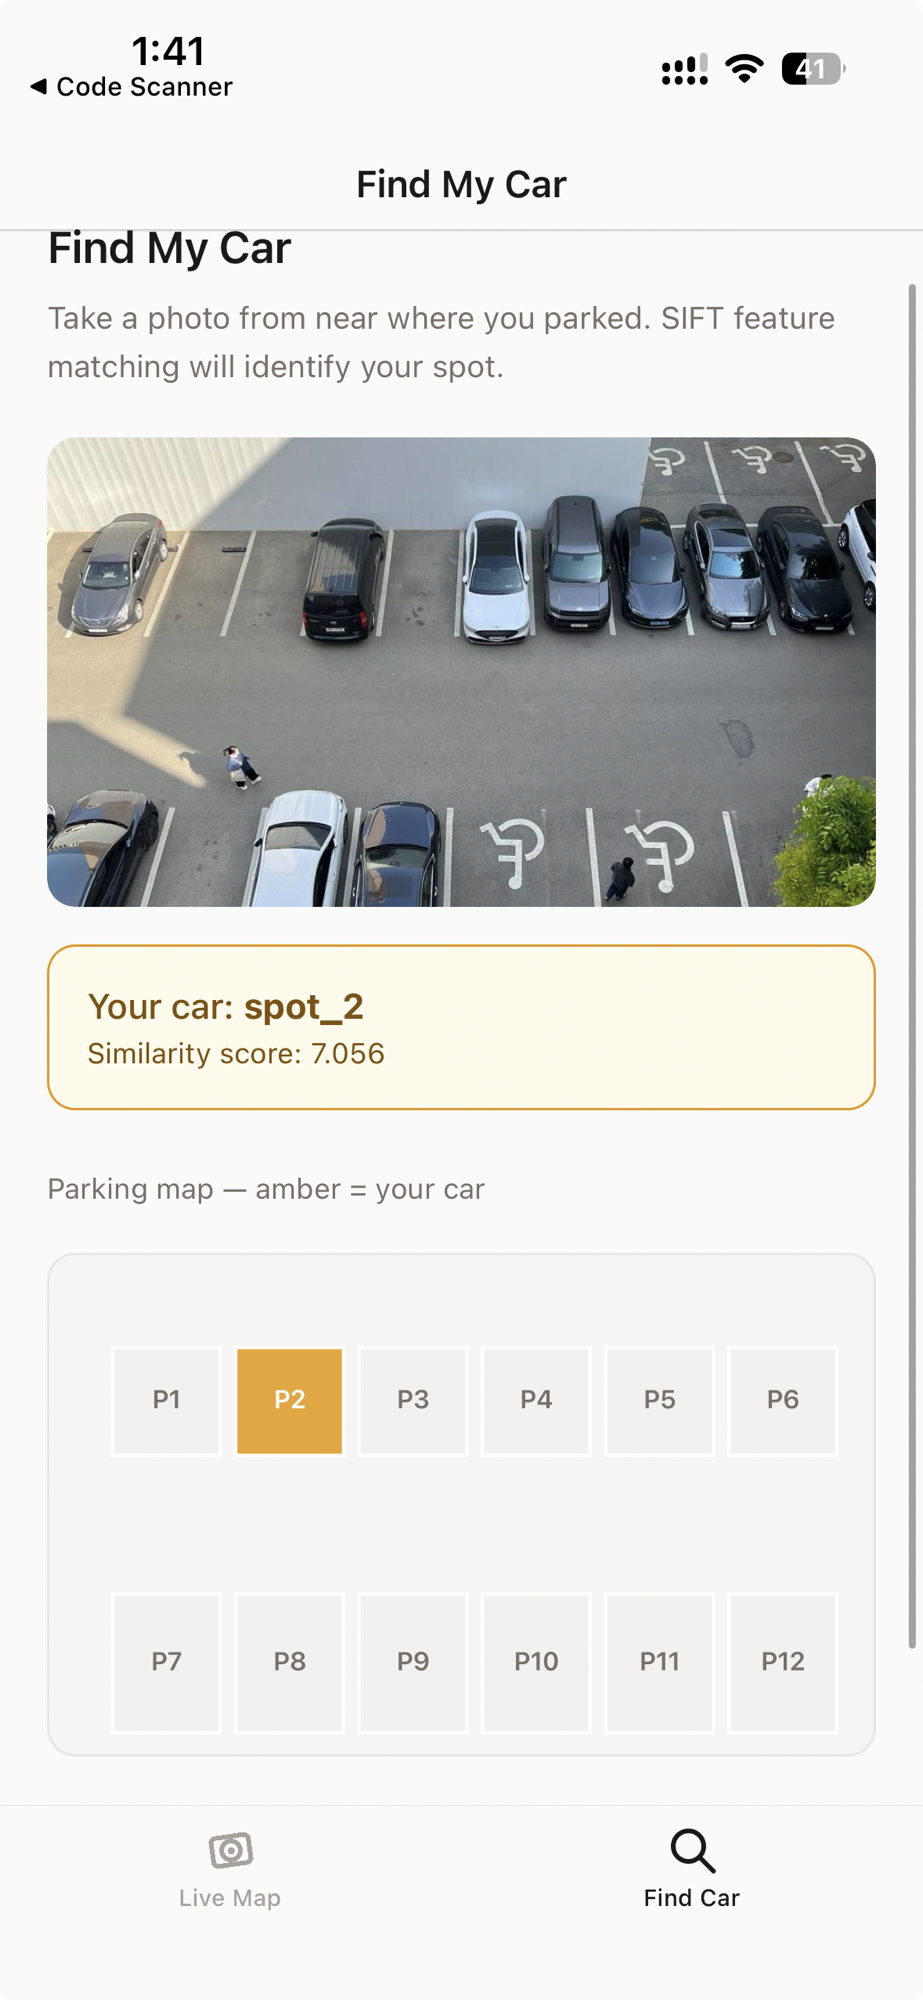
\includegraphics[width=0.6\linewidth]{figures/ui_find_my_car.png}
\caption{Find My Car (mobile): the localized spot highlighted in amber
after a driver photo is matched to the published layout.}
\label{fig:ui-fmc}
\end{figure}

\subsection{Case study: live occupancy counter bug}
\label{sec:casestudy}

During integration testing, the web dashboard displayed 55 free and 127
occupied spots against a 12-spot layout. The root cause was that the
counters aggregated \emph{every} entry of the raw \texttt{/status}
payload --- which can contain stale spot identifiers from earlier edge
runs --- while the map rendered only the published layout's spots. The
fix constrains the counters to the layout's spot identifiers, restoring
the invariant $\text{free} + \text{occupied} \leq \text{total}$ and
matching the mobile implementation, which was already correct. The
episode motivated a hardening recommendation: the backend should filter
\texttt{/status} responses to the currently published layout so all
clients receive consistent data by construction.

%%%%%%%%%%%%%%%%%%%%%%%%%%%%%%%%%%%%%%%%%%%%%%%%%%%%%%%%%%%%%%%%%%%%%%%%%%%%%%%%%
\section{Conclusion}
%%%%%%%%%%%%%%%%%%%%%%%%%%%%%%%%%%%%%%%%%%%%%%%%%%%%%%%%%%%%%%%%%%%%%%%%%%%%%%%%%

This project delivers an edge-based smart parking system that classifies
per-space occupancy from a single overhead camera and reports it as a few
hundred bytes of JSON, with no imagery leaving the device. The decisive
design choice was to pool each parking space along its annotated
quadrilateral and perspective-warp it before classification: that single
change lifted accuracy from a 90.9\,\% fixed-ROI baseline to 97.72\,\% on
ACPDS's held-out, unseen-lot test split --- matching the dataset paper's
ResNet50 baseline with the \emph{smallest} model variant --- and a
controlled ablation confirms the quadrilateral advantage holds on both
validation and test. Around the model, the system is a complete product:
owner setup, live web and mobile occupancy maps, and a photo-based
\emph{Find My Car} feature that localizes 21/21 queries correctly. Stage 2
runs at 155--858\,FPS across PyTorch, ONNX, and Core ML INT8 backends,
hundreds of times faster than the reporting cadence requires.

The full product path is validated automatically: an in-process smoke test
drives owner setup, map persistence, edge update, live status, and the
park/find round-trip against the real localizer, and the clients carry
contract tests for the layout, occupancy-counting, and park/find response
shapes.

Future work is narrow. Low-light recall is the weakest metric (93.5\,\%),
and luminance-aware augmentation is the natural remedy. The owner-setup
flow currently stores a precomputed layout rather than running
Structure-from-Motion on uploaded photos end-to-end; wiring that, with a
manual-correction fallback, would complete the configuration story. A
longer soak test and backend-side filtering of status payloads against the
published layout (the hardening from Section~\ref{sec:casestudy}) round out
the remaining engineering work.

{\small
\bibliographystyle{ieee_fullname}
\bibliography{references}
}

\end{document}
